% PREAMBLE Version 0.1

% DO NOT COMPILE THIS FILE ALONE

% Document classes
% ----------------
\documentclass[a4paper, 11pt, oneside]{article}
% \documentclass[a4paper,landscape]{article}

% Project structure
% -----------------
\usepackage{subfiles}

% Spacing, margins, etc.
% ----------------------
\usepackage{geometry}
\usepackage{float}
\usepackage{fullpage}
\usepackage{indentfirst}
\usepackage[francais]{babel}
% \usepackage[english]{babel}

% Encoding, characters, fonts, etc.
% ---------------------------------
\usepackage[T1]{fontenc}
\usepackage[utf8]{inputenc}
% \usepackage{upgreek}
\usepackage{eurosym}
\usepackage{amsfonts}
\usepackage{amssymb}
\usepackage{textcomp}

% Figures
% -------
\usepackage{graphicx}
% \usepackage{subfigure}

% Colors
% ------
% \usepackage{color}
\usepackage[table]{xcolor}

% URLs and refs
% -------------
% \usepackage{url}
% \usepackage{hyperref}
% \usepackage[bottom]{footmisc}
% \usepackage[all]{hypcap}

% Environments
% ------------
\usepackage{amsmath}
\usepackage{amsthm}
\usepackage{array}
\usepackage{tabularx}
\usepackage{enumerate}
\usepackage{enumitem}
\usepackage{listings}
\usepackage{framed}
\usepackage[framed]{matlab-prettifier}
\usepackage{booktabs}
\usepackage{algorithm}
\usepackage{algorithmic}

% =================================================================================
%                                   New commands
% =================================================================================



\renewcommand{\thesubsection}{\alph{subsection})}
\renewcommand{\thesubsubsection}{\roman{subsubsection})}
\usepackage{clrscode3e}

\begin{document}

\subfile{titlepage.tex}

\section{Répartition des cases} %1
%Ton boulot drewdrew <3
\subsection{} %a
Une approche exhaustive consisterait à calculer toutes les possibilités de répartition des images puis de chercher celui avec le coût minimal. \\

\paragraph{Si il y a 1 image a répartir,} il n'y a qu'une possibilité.
	\begin{itemize}
		\item 1 image sur la première ligne
	\end{itemize}
\paragraph{Si il y a 2 images à répartir,} il y a deux cas possible.
	\begin{itemize}
		\item 2 images sur la première ligne
		\item 1 image sur la première ligne et une sur la seconde.
	\end{itemize}

\paragraph{Si il y a 3 images à répartir,} il y a 4 possibilités.
	\begin{itemize}
		\item 3 images sur la première ligne
		\item 2 images sur la première ligne et une sur la seconde
		\item 1 images sur la première ligne et 2 sur la seconde
		\item 1 image par ligne\\
	\end{itemize}
	
À chaque ajout d'une image, on multiplie par deux le nombre de possibilités de répartitions. Dans une cas plus générale on peut dire que la complexité est de $2^n-1$ avec $n$ le nombre d'images à répartir.

\subsection{} %b
	
\[c(i) = 
\left\{
\begin{array}{l l l}
C(0,0) &  & i = 0\\
min_{0 \leq k \leq i}(c(k) + C(k, i)) &  & i > 0\\
\end{array}
\right.
\]


	où $C(i,j)$ est le coût pour mettre 	une image i et j sur la même ligne. 
	
\subsection{} %c

\begin{figure}[H]
	\centering
	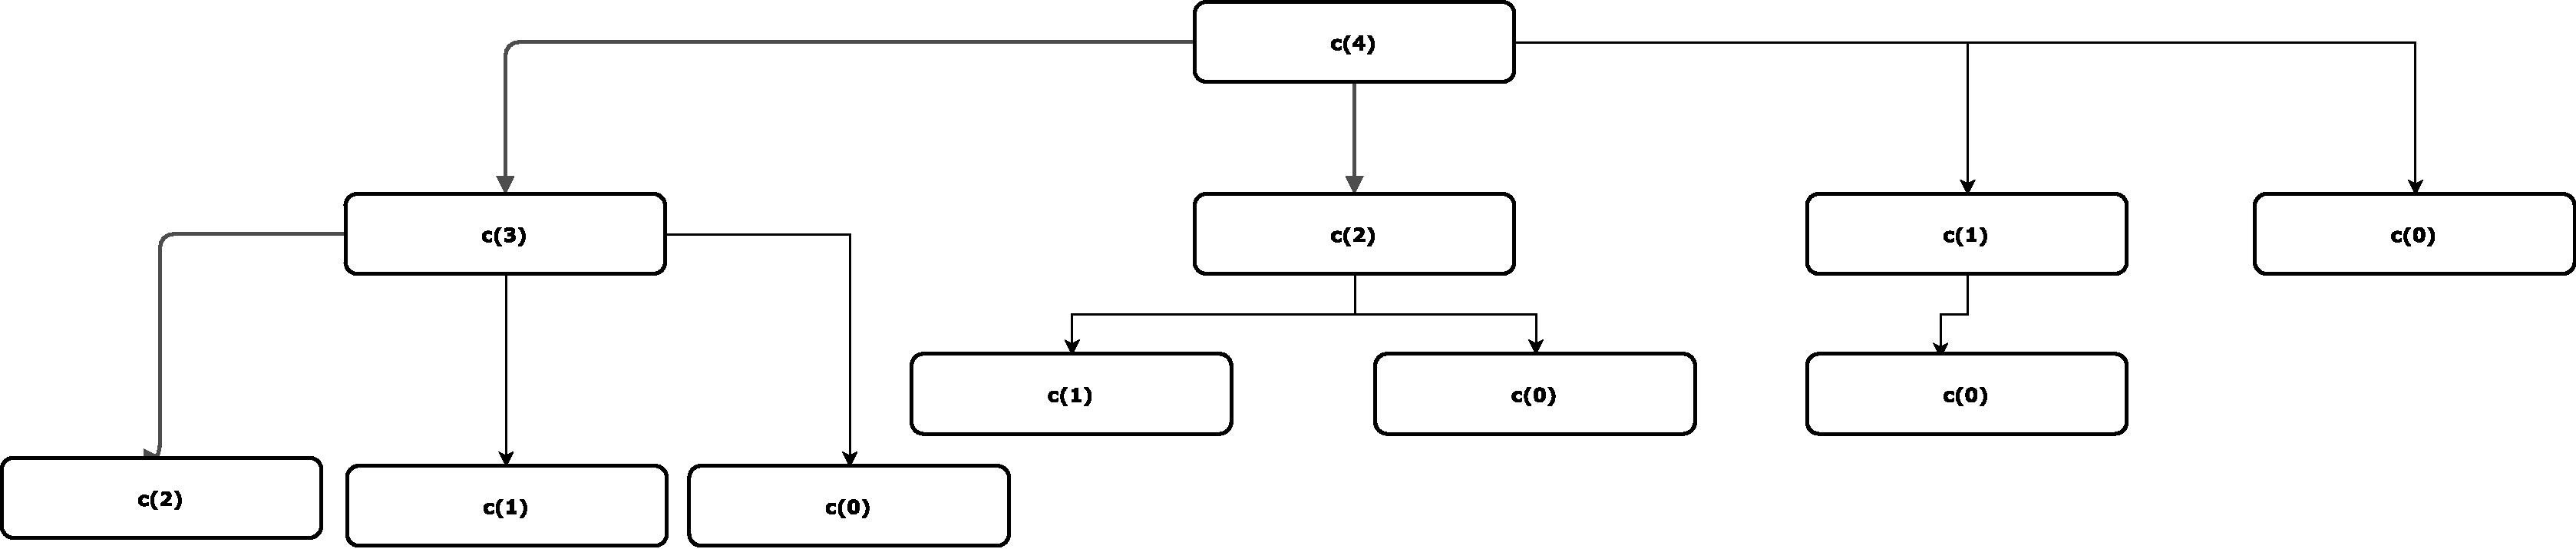
\includegraphics[width=1\linewidth]{diagram.pdf}
	\caption{Graphe des appels récursifs}
	\label{cost}
\end{figure}

\subsection{} %d


\begin{codebox}
\Procname{$\proc{Optimal}(j, nbImages)$}
\li \If $j < nbImages + 1$
	\Do
	\li \If $j == 0$
		\Do
		\li $optimalCost[j] = 0$
	\li \Else
		
		\li $optimalCost[j] = + \infty$
		\li \For $i = 1$ \To $j$
		\Do
			\li \If $(optimalCost[i - 1] + costMatrix[i - 1][j - 1] < optimalCost[j])$
			\Do
				\li $optimalCost[j] = optimalCost[i - 1] + costMatrix[i - 1][j - 1]$
				\li $mem[j] = i$
				
			\End
		\End \End
	\li $optimal(j + 1, nbImages)$
	\End
\li \Return $mem$
	
\end{codebox}


\subsection{} %e
	La complexité temporelle est $O(n^2)$ et la complexité spatiale dépends de costMatrix

\setcounter{section}{0}

\section{Calcul de la couture d'énergie minimale} %1
%Mon boulot
\subsection{} %a
Une approche exhaustive consisterait à calculer le coût de tous les chemins possibles puis de chercher celui avec le coût minimal.
Pour atteindre le pixel (i, j), i étant la dernière ligne:

Si la hauteur = 1, 1 chemin possible.

Si la hauteur = 2, 3 chemins possibles.\footnote{Si le pixel est au bord de l'image alors il n'y a que 2 chemins possibles, mais on ne va pas considérer ce cas ici pour plus de simplicité}

Si la hauteur = 3, $3*3=9$ chemins possibles.

Si la hauteur = n, $3*3*...=3^{n-1}$ chemins possibles.

L'approche exhaustive est donc bien de complexité exponentielle.
\subsection{} %b
Cas de base, $i = 0$, $j \in [0, largeur - 1]$ ;

 $C(i, j)$ = $E(i, j)$
\bigbreak
$\forall i > 0, j \in [0, largeur - 1]$ tels que $C(i - 1, j -1)$, $C(i - 1, j)$ et $C(i - 1, j + 1)$ sont définis :

$C(i, j) = E(i, j) + min(C(i - 1, j -1), C(i - 1, j), C(i - 1, j + 1))$\footnote{Si j - 1 ou j + 1 dépassent les limites de l'image, on n'en tient pas compte dans le calcul du minimum.}
\subsection{} %c
\begin{figure}[H]
	\centering
	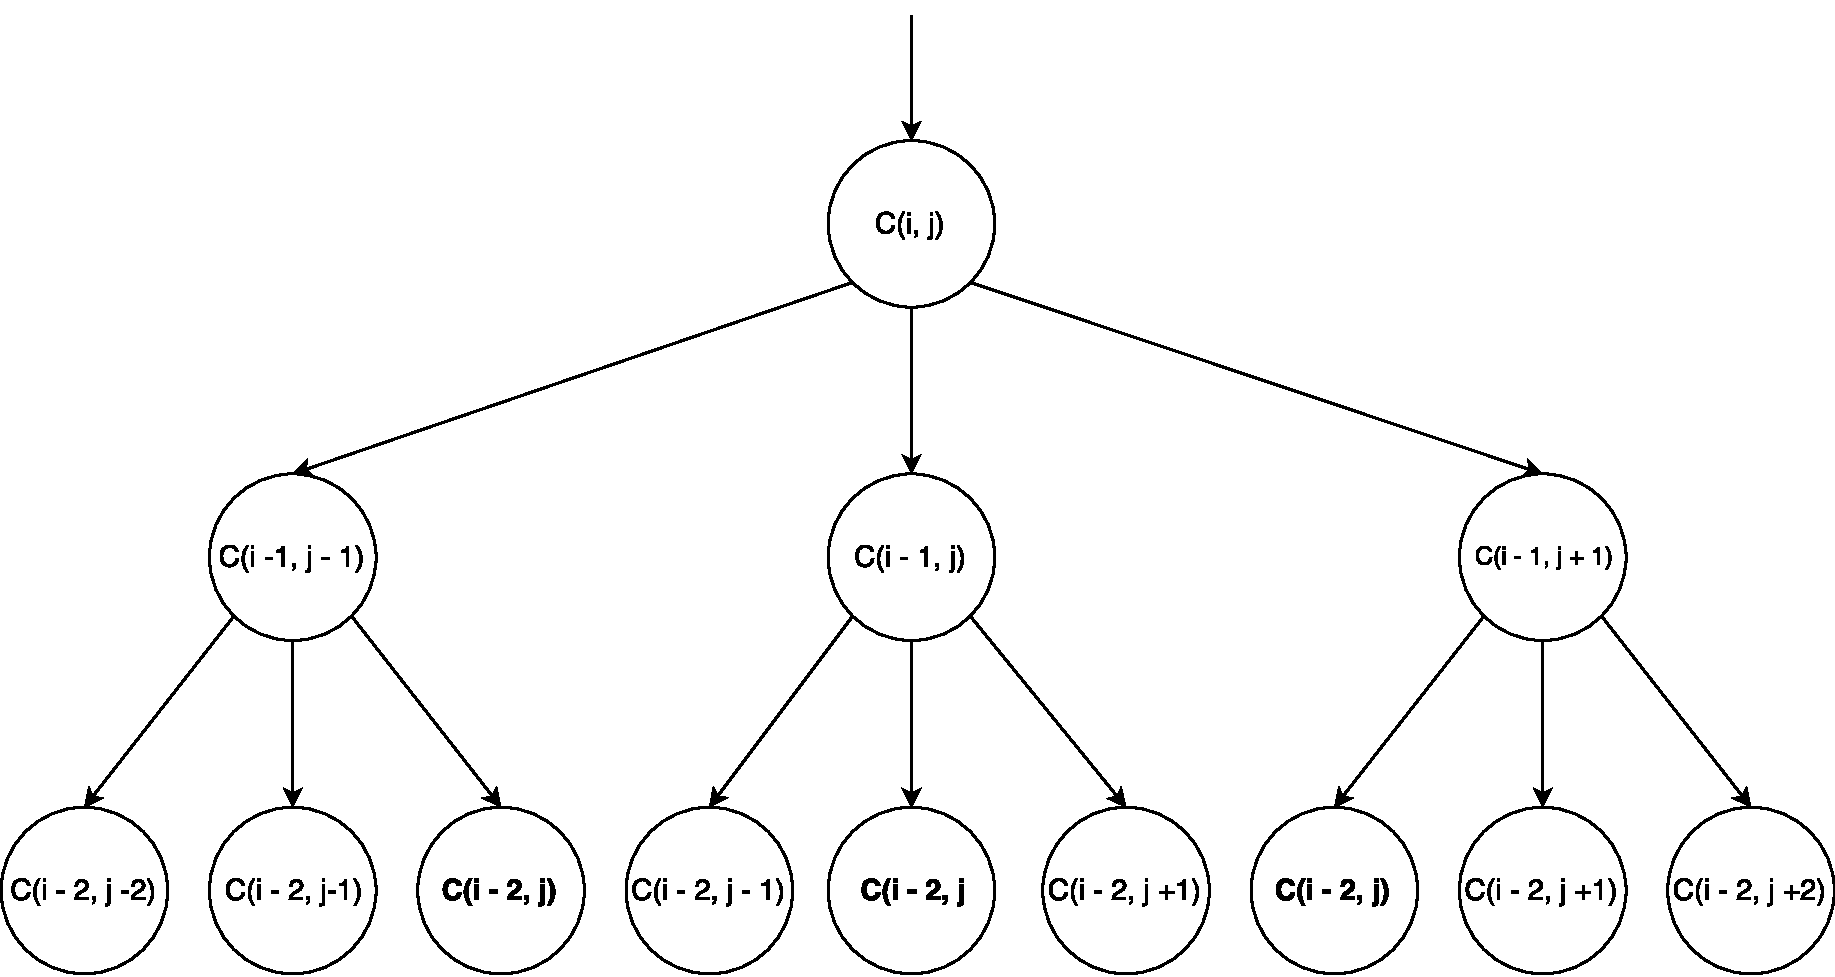
\includegraphics[width=1\linewidth]{cost.pdf}
	\caption{Graphe des appels récursifs}
	\label{cost}
\end{figure}

On peut voir dans la figure \ref{cost} que l'on effectue plusieurs fois le même appel (en gras). Afin de ne pas faire inutilement des calculs, on tâchera de retenir les valeurs déjà calculées.

\subsection{} %d
\begin{codebox}
\Procname{$\proc{Cost}(energy)$}
\li \For $j = 1$ \To $width$
\Do
\li 	$cost[1][j] = energy[1][j]$
\End
\li \For $i = 2$ \To $heigth$
\Do 
\li 	\For $j = 1$ \To $width$
 		\Do
\li 		\If $j - 1> 1$
			\Do 
\li 			$left = cost[i - 1][j - 1]$
\End
\li 		$mid = cost[i - 1][j]$
\li 		\If $j + 1< width$
			\Do 
\li 			$right = cost[i - 1][j + 1]$
\End
\li \Comment Si left ou right n'est pas défini, on n'en tient pas compte
\li 		$cost[i][j] = energy[i][j] + min(left, mid, right)$
	\End
\End
\li \Return $cost$
\end{codebox}
$energy$ est un tableau de taille $heigth * width$ contenant l'énergie de chaque pixel.

\subsection{} %e
Pour une image de taille n * m, la complexité est $\Theta(n * m)$.

L'espace mémoire utilisé est constant.

\section{Fonctions de réduction et d'élargissement d'une image} %2
%Mon boulot aussi
\subsection{Implémentation} %a
Pour chacune des fonctions, on utilise deux tableaux de même taille que l'image : $energy$ et $sum$. 
On effectue une boucle $k$ fois :

On calcule l'énergie de chaque pixel et on la place dans $energy$.
Ensuite on calcule le coût de chaque pixel, et on enregistre les résultats dans $sum$.
Finalement on cherche le minimum dans la dernière ligne de $sum$ et parcourt $sum$ du bas vers le haut à partir de ce point afin de reconstituer la couture d'énergie minimale que l'on enregistre dans $seam$.

Dans le cas d'un élargissement, on note dans un tableau $marked$, de même taille que l'image, les pixels de la couture d'énergie minimale.

Ensuite on recopie l'image en enlevant les pixels de la couture d'énergie minimale, on a donc une image réduite d'un pixel en largeur.
\bigbreak
Après cette boucle le programme se termine et renvoie la nouvelle image réduite $k$ fois dans le cas d'une réduction. 

S'il s'agit d'un élargissement, on recopie l'image originale et pour chaque pixel marqué on ajoute un pixel à sa droite comme expliqué dans l'énoncé. On retourne ensuite cette image de k pixels plus large.
\subsection{Complexités} %b
Pour les deux fonctions la complexité en espace est constante puisqu'on modifie directement dans les images et les tableaux.
La complexité de \textbf{reduceImageWidth} est $\Theta(k*n*m)$.

La complexité de \textbf{increaseImageWidth} est $\Theta(k*n*m)$ si k est inférieur à 20\% de la largeur originale de l'image. Si k est supérieur à 20\%, on devra appeler $n$ fois la fonction pour ne pas dépasser $k > 20\% * m$.
\end{document}
